\documentclass[tikz,border=20pt]{standalone}
\usetikzlibrary{positioning, arrows.meta}

\begin{document}

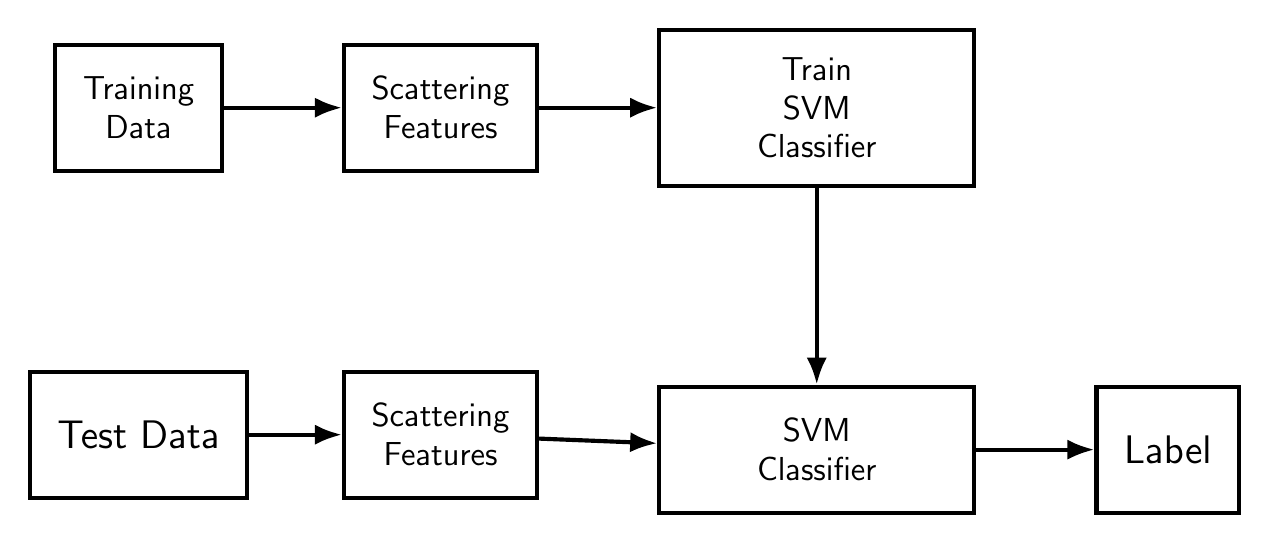
\begin{tikzpicture}[
    node distance=2.5cm and 1.5cm, %% Vertical and horizontal distance
    box/.style={
        rectangle,
        draw=black,
        line width=1.5pt,
        align=center,
        fill=white,
        font=\sffamily\large,
        inner sep=10pt,
        minimum height=1.6cm
    },
    arrow/.style={
        ->,
        >=Latex,
        line width=1.5pt
    },
    caption/.style={
        below=3pt,
        font=\sffamily,
        align=center
    }
]

%% Top Row Nodes
\node[box] (train_data) {Training\\Data};
\node[box, right=of train_data] (train_sf) {Scattering\\Features};
\node[box, right=of train_sf, minimum width=4cm] (train_svm) {Train\\SVM\\Classifier};

%% Bottom Row Nodes
\node[box, below=of train_data] (test_data) {\Large Test Data};
\node[box, below=of train_sf] (test_sf) {Scattering\\Features};
\node[box, below=of train_svm, minimum width=4cm] (svm_class) {SVM\\Classifier};
\node[box, right=of svm_class] (label) {\Large Label};


%% Horizontal Connections
\draw[arrow] (train_data) -- (train_sf);
\draw[arrow] (train_sf) -- (train_svm);

\draw[arrow] (test_data) -- (test_sf);
\draw[arrow] (test_sf) -- (svm_class);
\draw[arrow] (svm_class) -- (label);

%% Vertical Connection
\draw[arrow] (train_svm) -- (svm_class);

\end{tikzpicture}

\end{document}